\subsection{Instagram}

Instagram là một mạng xã hội chuyên chia sẻ hình ảnh và video trên IOS, Android và Windows phone, bản thân nó được thiết kế dựa trên cơ sở sáng tạo ra những bức ảnh đẹp và thu hút. Đồng thời, nó cũng cung cấp rất nhiều các chế độ chỉnh sửa ảnh và video khác nhau theo sở thích của người dùng.\\ \par

Năm 2010, Instagram nhanh chóng trở thành một trong những mạng xã hội phát triển nhất. Đến năm 2012, Instagram được Facebook mua lại, cuộc sáp nhập này giúp cho Instagram đạt được con số tăng trưởng người dùng nhanh hơn cả Facebook, Twitter hay Pinterest. Chỉ sau 1 năm sát nhập với 
 Facebook, mạng xã hội Instagram đã đạt tới con số 150 triệu người dùng mỗi tháng.\\ \par
\par

Instagram cũng được đánh giá là sử dụng rất đơn giản. Những người lớn tuổi cũng có thể dễ dàng sử dụng nó, chỉ cần chạm vào biểu tượng máy ảnh sau đó chụp cho mình một vài tấm ảnh rồi tải lên là được. Còn đối với giới trẻ hiện nay thì Instagram đã không còn quá xa lạ, đây là ứng dụng phổ biến, kênh truyền thông hiệu quả, có khả nắng thúc đẩy tương tác rất tốt. Vì thế Instagram rất dễ dàng tiếp cận với người dùng trên toàn cầu. \\ \par

Bạn có thể thỏa thích chia sẻ hình ảnh một cách an toàn với Instagram. Bạn có thể lựa chọn nhiều hình thức để chia sẻ hình ảnh như: Chia sẻ cho bạn bè hay thiết lập quyền riêng tư chỉ riêng bạn thấy. Hoặc bạn có thể sử dụng chức năng Share Direct để share hình ảnh này với duy nhất một người. Chứng tỏ Instagram rất tôn trọng việc riêng tư của người dùng.\\ \par 

Phía trên là một vài thông tin cơ bản, bên cạnh đó thì Instagram còn cung cấp rất nhiều tính năng nổi bật, chúng ta cùng tìm hiểu cụ thể về mạng xã hội này.\\ \par

\newpage
\textbf{Những tính năng nổi bật của Instagram:}
\begin{itemize}
    \item \textbf{Xem và chia sẻ ảnh, video.} Một bức ảnh, video đơn giản có thể nói lên hết những suy nghĩ và cảm xúc của bạn. Bạn dễ dàng xem và chia sẻ những bức ảnh, video thay lời muốn nói trên ứng dụng Instagram. Đặc biệt, bạn có thể xem lại những bức ảnh bạn đã like dễ dàng từ vài tuần đến vài tháng trước. Ngoài ra, bạn có thiết lập quyền riêng tư khi chia sẻ ảnh và video trên ứng dụng, bạn dễ dàng quản lý ai được quyền xem và like những bức ảnh, video của bạn.\par
    \begin{figure}[h!]
        \centering
        
\includegraphics[width=6cm]{Images/chapter 2/instagram/post_app.jpg}
        \caption{Bài đăng trên ứng dụng di động}
        \label{fig:my_label}
    \end{figure}
  
    \begin{figure}[h!]
        \centering
        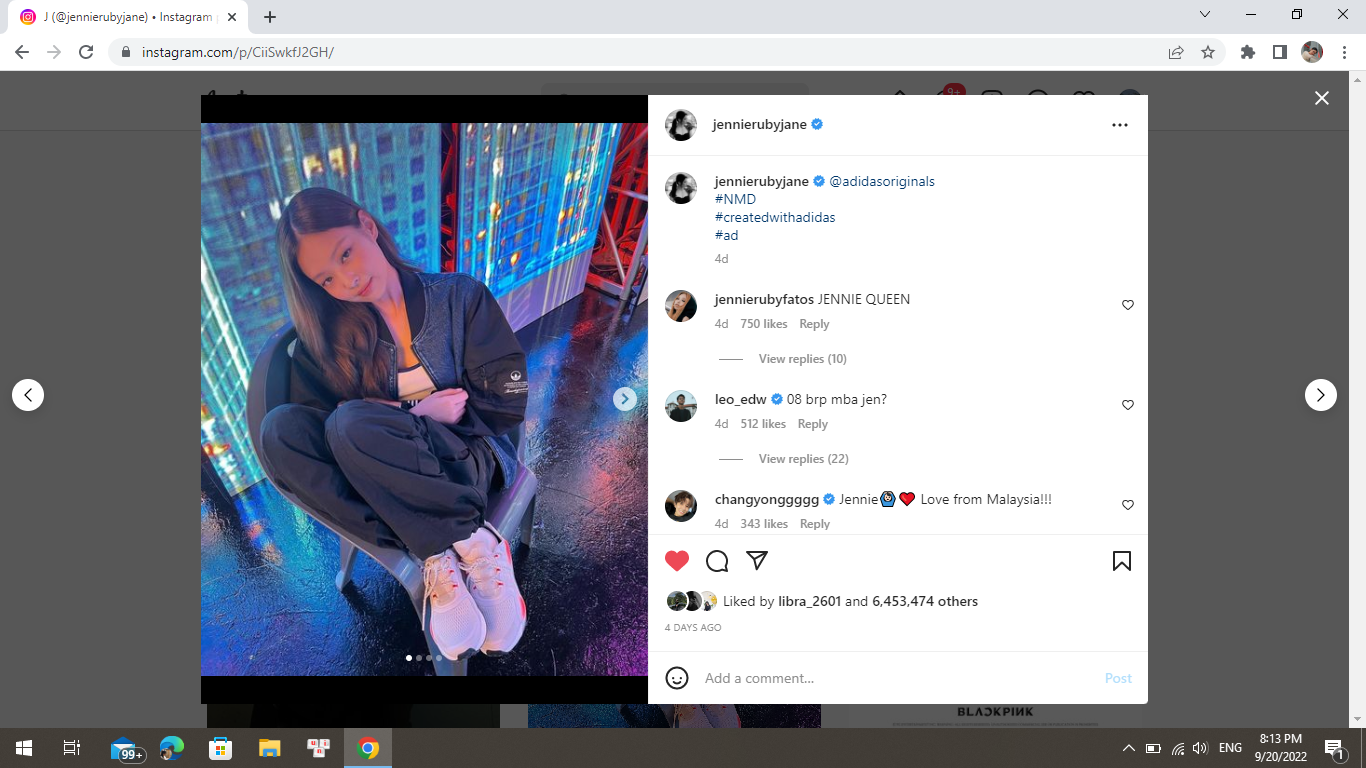
\includegraphics[width=12cm]{Images/chapter 2/instagram/post_web.png}
        \caption{Bài đăng trên web}
        \label{fig:my_label}
    \end{figure}
\\
\newpage
    \item \textbf{Công cụ tạo ảnh, video sống động.} Bạn dễ dàng chỉnh sửa ảnh và video bằng Instagram để có những bức ảnh đẹp nhất trước khi đăng lên bảng tin của mình. Với những công cụ chỉnh sửa đơn giản như các bộ lọc, hiệu ứng, bóng mờ, làm rõ nét, chỉnh sửa màu sắc… để có bức ảnh đẹp nhất.\\
\newpage
    \begin{figure}[h!]
        \centering
        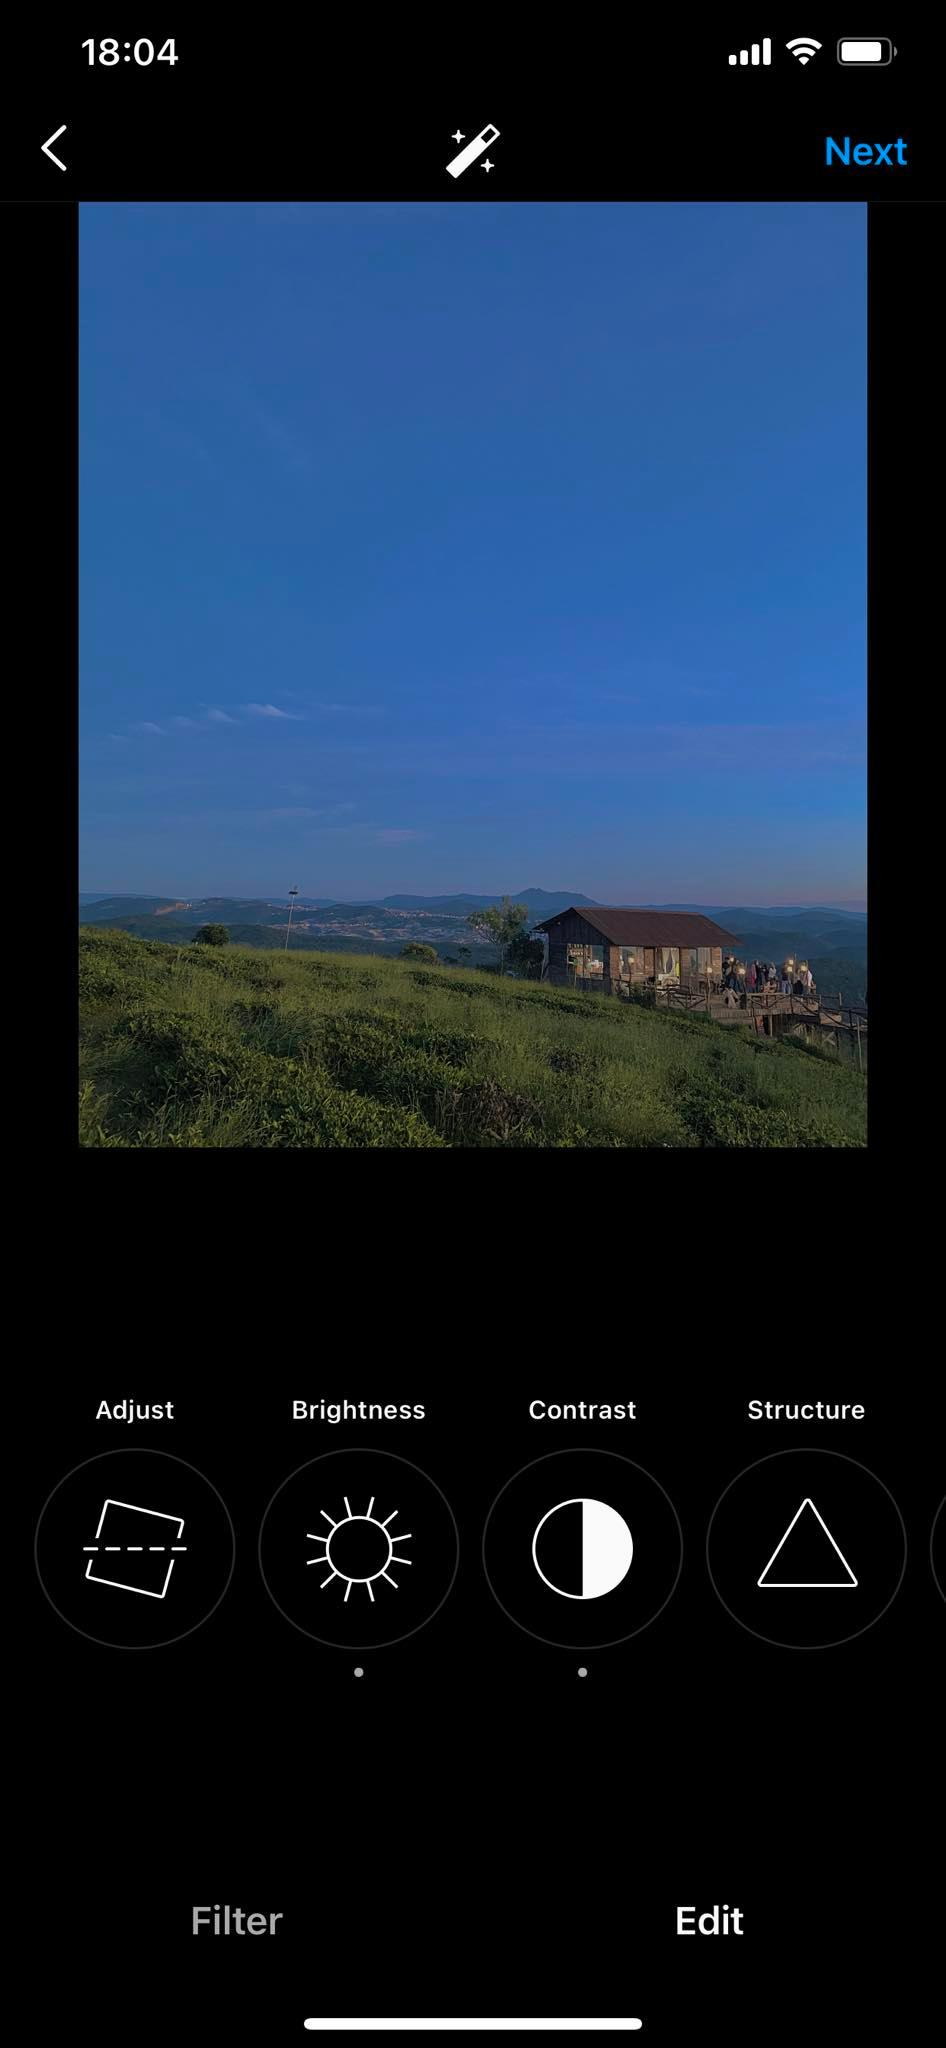
\includegraphics[width=7cm]{Images/chapter 2/instagram/edit_app.jpg}
        \caption{Chỉnh sửa ảnh trên ứng dụng di động}
        \label{fig:my_label}
    \end{figure}
    
    \begin{figure}[h!]
        \centering
        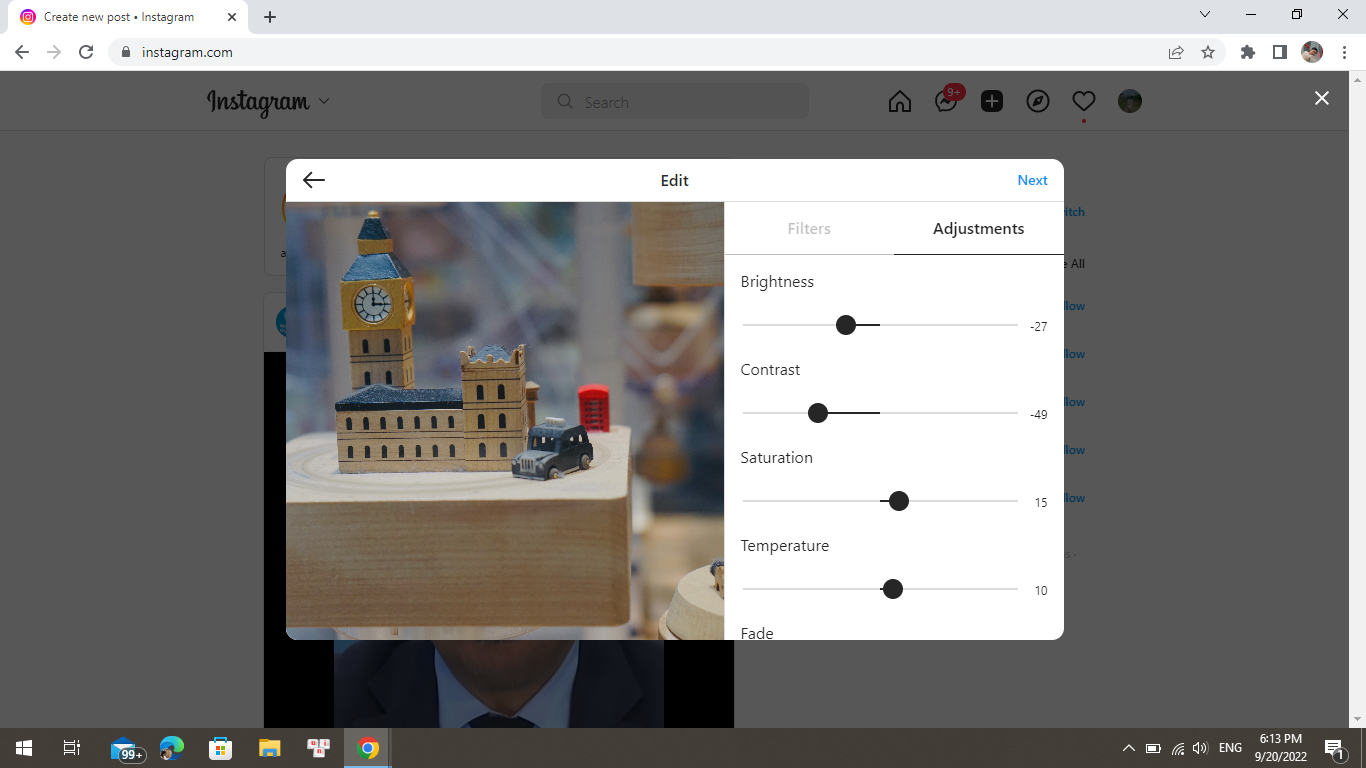
\includegraphics[width=13cm]{Images/chapter 2/instagram/edit_web.png}
        \caption{Chỉnh sửa ảnh trên web}
        \label{fig:my_label}
    \end{figure}
\\
\newpage
    \item \textbf{Tìm kiếm và khám phá nhiều nội dung từ cộng đồng, Reels.} Instagram là ứng dụng mạng xã hội phát triển rộng rãi trên toàn thế giới. Vì vậy, cũng như các ứng dụng mạng xã hội khác, bạn dễ dàng tìm kiếm và khám phá mọi thứ từ những bức ảnh, video trong được chia sẻ trên Instagram.\\
\newpage
    \begin{figure}[h!]
        \centering
        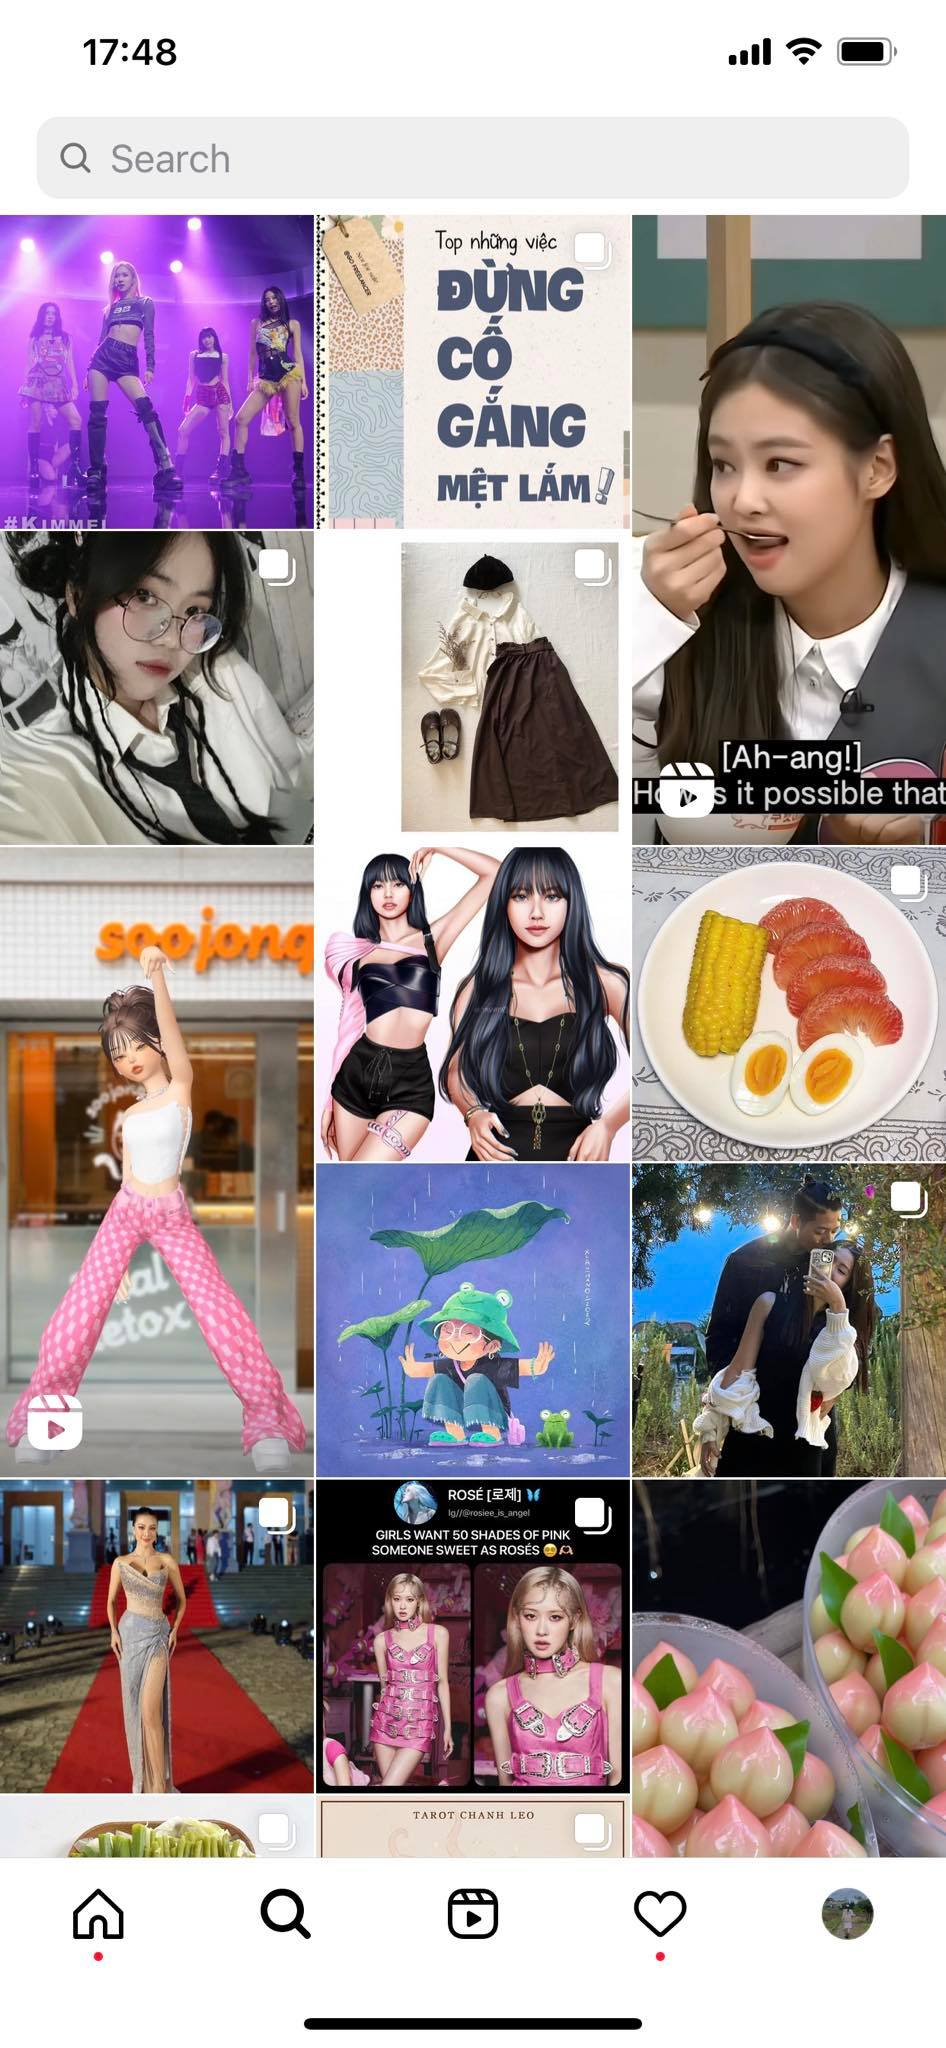
\includegraphics[width=7cm]{Images/chapter 2/instagram/search_app.jpg}
        \caption{Tìm kiếm và khám phá nội dung trên ứng dụng di động}
        \label{fig:my_label}
    \end{figure}\
    
    \begin{figure}[h!]
        \centering
        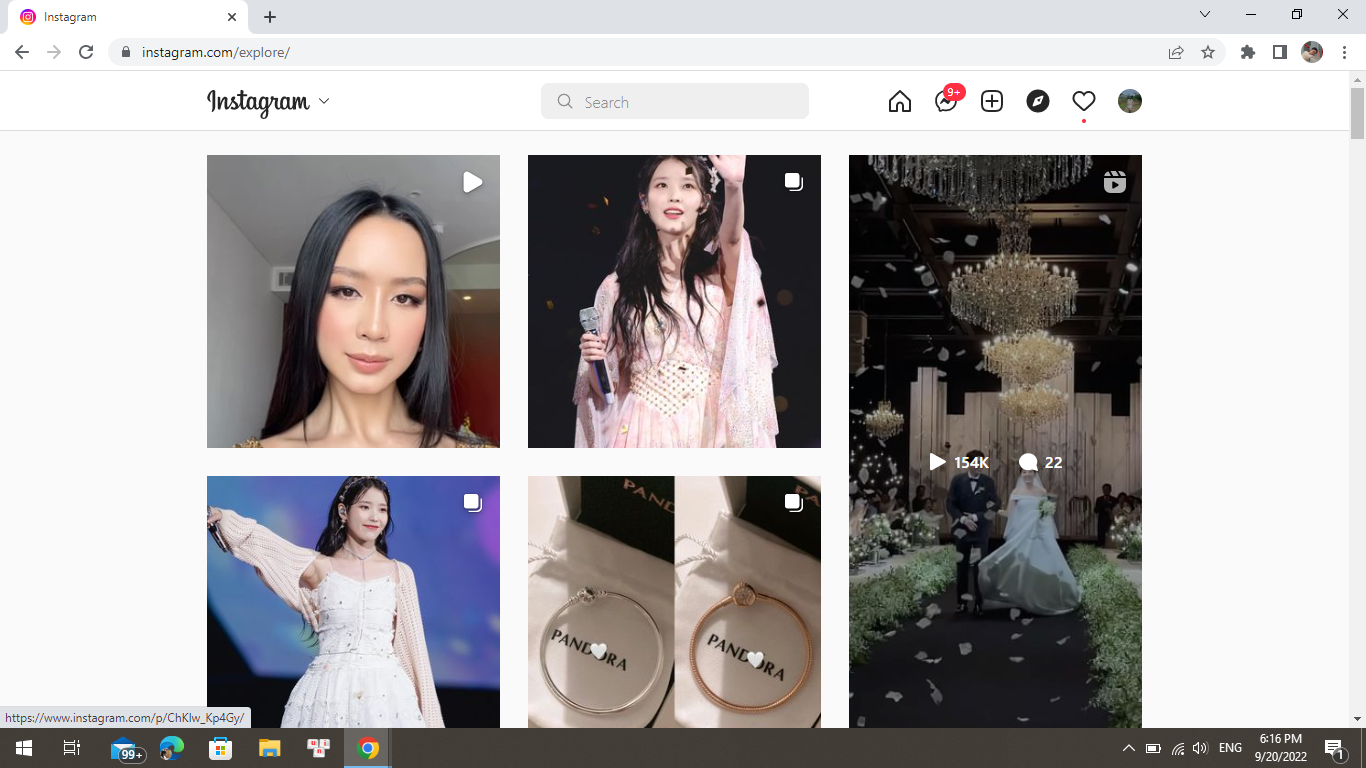
\includegraphics[width=13cm]{Images/chapter 2/instagram/search_web.png}
        \caption{Tìm kiếm và khám phá nội dung trên web}
        \label{fig:my_label}
    \end{figure}
\\
\newpage
    Ngoài ra reels của Instagram cũng được đánh giá là nơi chia sẻ video rất hot hiện nay.
    \begin{figure}[h!]
        \centering
        
\includegraphics[width=7cm]{Images/chapter 2/instagram/reel_app.jpg}
        \caption{Reels trên ứng dụng di động}
        \label{fig:my_label}
    \end{figure}
\\
\newpage
    \item \textbf{Đăng story và phát live stream dễ dàng.} Để chia sẻ những khoảnh khắc đáng nhớ, những hiệu ứng có sẵn của ứng dụng sẽ giúp bạn tạo ra những video đẹp nhất ngay từ lúc quay. Với chức năng đăng story, bạn dễ dàng chia sẻ những thước phim, video đó lên bảng tin của mình, ngoài ra còn có tính năng live stream đến bạn bè và những người theo dõi bạn. Khi phát trực tiếp xong bạn có thể xóa hoặc đăng tải video lên bản tin Instagram của mình để người khác xem lại.\\ \par
    \begin{figure}[h!]
        \centering
        
\includegraphics[width=7cm]{Images/chapter 2/instagram/story_app.jpg}
        \caption{Story trên ứng dụng di động}
        \label{fig:my_label}
    \end{figure}
    \begin{figure}[h!]
        \centering
        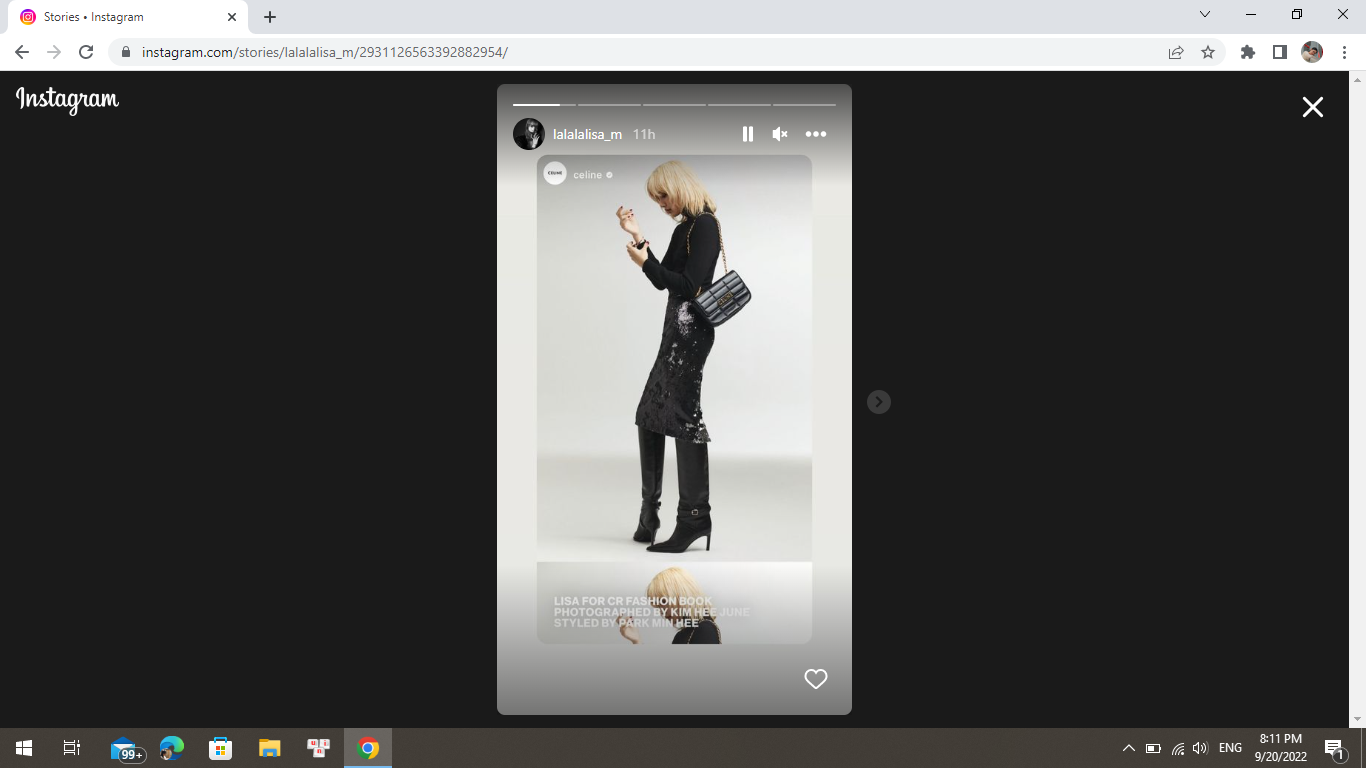
\includegraphics[width=13cm]{Images/chapter 2/instagram/story_web.png}
        \caption{Story trên web}
        \label{fig:my_label}
    \end{figure}
\\
\newpage
    \item \textbf{Tích hợp công cụ nhắn tin.} Bạn có thể nhắn tin, trò chuyện cùng bạn bè người thân, với những người mình yêu quý và có chung sở thích qua Instagram. Ngoài ra, bạn có thể sử dụng tính năng gọi video call để trò chuyện miễn phí ngay trên ứng dụng.
\end{itemize}

\subsubsection{Ưu điểm và nhược điểm}
\subsubsubsection{Ưu điểm}
\textbf{Những điểm nổi bật của Instagram so với facebook:}
\begin{itemize}
    \item Chỉ với một bức ảnh bạn bè có thể đoán được tâm trạng của bạn đang vui hay buồn.
    \item Nếu như Facebook chủ yếu là chia sẻ cảm xúc của bạn bằng những status thì Instagram chỉ cần một bức ảnh mọi người đã biết bạn đang cảm thấy như thế nào. Đây chính là một yếu tố khiến Instagram thu hút hơn Facebook.
    \item Hiện tại Instagram đã cập nhật tính năng cho phép bạn ghi lại hình ảnh của bạn trong vòng 15 giây. Bạn có thể ghi lại một video khoảng 15 giây và nói một điều gì đó thú vị. Hiện tại Instagram chưa phát triển hết khả năng video nhưng trong những thời gian tới có lẽ chức năng quay video sẽ có thời gian dài hơn 15 giây.
    \item Instagram sử dụng rất đơn giản, người lớn tuổi cũng có thể dễ dàng sử dụng. Bạn chỉ cần bấm vào Instagram, chạm vào biểu tượng máy ảnh, chụp một tấm và nhấn tải ảnh lên.
    \item Instagram được ưa thích hơn facebook là nhờ 19 hiệu ứng chỉnh sửa ảnh. Bạn có thể tìm thấy một hiệu ứng hoàn hảo cho bất kỳ bức ảnh nào của mình. Những hiệu ứng này chắc chắn sẽ làm bạn cảm thấy hào hứng và hài lòng.
    \item Instagram có ứng dụng Emoji giúp bạn thêm một khuôn mặt cười hay ngón tay hướng lên trên để thể hiện cảm xúc khi bức ảnh của bạn bè bạn đăng lên mà không biết phải bình luận như thế nào.
    \item Instagram cũng cho phép bạn bè của bạn biết rằng: Bạn đang tồn tại, bạn đang làm gì? Bạn đang đi đâu?
    \item Với Instagram, bạn có thể nhìn thế giới qua đôi mắt của người khác, điều đó thực sự rất tuyệt vời.
    \item Khi dùng Instagram bạn không phải bắt gặp những tin spam liên quan đến quảng cáo. Tại đây, bạn sẽ được thỏa sức định hình phong cách cá nhân của mình. Ngay cả khi phong cách đó là những bức ảnh không sử dụng hiệu ứng hay chỉnh sửa.
\end{itemize}
\\ \par
\newline
\textbf{Với những phân tích và khảo sát, có thể đúc kết được Instagram có các ưu điểm như sau:}
\begin{itemize}
    \item Là một mạng xã hội lớn, phổ biến rộng rãi, được lượng lớn người dùng ưu chuộng.
    \item Hình ảnh có khả năng gợi lên cảm xúc, hấp dẫn hơn các hình thức tương tác khác
    \item Công cụ tiếp thị tốt, nhiều cửa hàng ảo sử dụng nền tảng này để quảng bá sản phẩm của họ.
    \item Chú trọng về quyền riêng tư và bảo mật. Đây là một trong những lợi thế quan trọng của Instagram.
    \item Ứng dụng hoàn toàn miễn phí cho người dùng.
    \item Phương tiện giao tiếp tốt với các tính năng gọi, call video, phát livestream.
\end{itemize}
\subsubsubsection{Nhược điểm}
\textbf{Bên cạnh những ưu điểm đã phân tích, còn tồn tại một số nhược điểm:}
\begin{itemize}
    \item Instagram được thiết kế dành cho ứng dụng là chủ yếu, đối với phiên bản trên web thì Instagram không cung cấp nhiều dịch vụ như ứng dụng di động.
    \item Không tương thích với tất cả các hệ điều hành. Instagram chỉ khả dụng trên IOS, Android và Windows Mobile, điều này không bao gồm những người có thiết bị có hệ thống BlackBerry, OS và Linux.
    \item Khả năng trộm cắp hình ảnh. Khi đăng tải những  bức ảnh đẹp, chất lượng và chuyên nghiệp lên mạng xã hội, đặc biệt là mạng xã hội phát triển như Instagram thì việc bị đánh cắp hình ảnh mà không có sự đồng ý của chính chủ là rất phổ biến. 
    \item So với các mạng xã hội như Facebook, zalo thì Instagram không cung cấp tính năng group chat. Bạn chỉ có thể chat trực tiếp với 1 người.
    \item Instagram chứa nhiều trang cửa hàng ảo, dẫn tới việc quảng cáo nhiều, có khi thông tin sai lệch.
    \item Giống với các mạng xã hội khác thì Instagram còn có tiềm năng gây nghiện cho người dùng, dẫn tới phụ thuộc vào mạng xã hội.
\end{itemize}